\documentclass[border=8pt]{standalone}

% Visual reference for the OpenTikZ palette (reference/color-palettes/color-palettes.md).
\usepackage{tikz}

% --- palette: light / default (canonical, Okabe-Ito) ---
\definecolor{otblue}{HTML}{0072B2}
\definecolor{otorange}{HTML}{E69F00}
\definecolor{otteal}{HTML}{009E73}
\definecolor{otpurple}{HTML}{CC79A7}
\definecolor{otgray}{HTML}{5A5A5A}
% --- palette: dark-tuned (same roles, brighter for dark backgrounds) ---
\definecolor{otblueDk}{HTML}{56B4E9}
\definecolor{otorangeDk}{HTML}{E69F00}
\definecolor{ottealDk}{HTML}{2EBE9B}
\definecolor{otpurpleDk}{HTML}{E08FBE}
\definecolor{otgrayDk}{HTML}{B3B3B3}
\definecolor{otpaper}{HTML}{1E1E1E}

\begin{document}
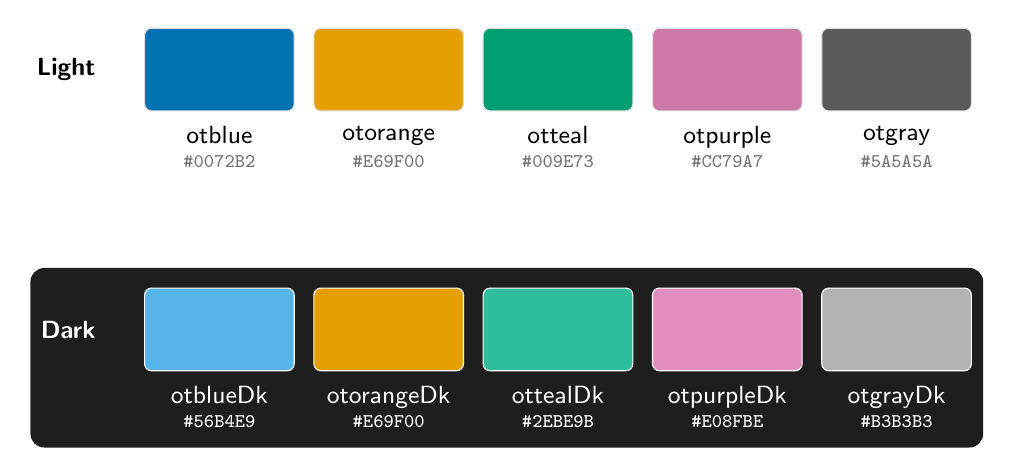
\begin{tikzpicture}[
    swatch/.style={
      minimum width=1.9cm, minimum height=1.05cm,
      rounded corners=2.5pt, draw=black!12, line width=0.4pt,
    },
    swname/.style={font=\sffamily\small, anchor=north},
    swhex/.style={font=\ttfamily\scriptsize, anchor=north},
    rowlbl/.style={font=\sffamily\bfseries\small, anchor=east},
  ]
  \def\dx{2.15}      % horizontal step between swatches
  \def\rightedge{4*\dx+1.1}

  % ===== light row =====
  \node[rowlbl] at (-1.45, 0) {Light};
  \foreach \i/\c/\h in {%
      0/otblue/0072B2, 1/otorange/E69F00, 2/otteal/009E73,
      3/otpurple/CC79A7, 4/otgray/5A5A5A} {
    \node[swatch, fill=\c] (s) at (\i*\dx, 0) {};
    \node[swname, text=black]   at ([yshift=-0.06cm]s.south) {\c};
    \node[swhex,  text=black!55] at ([yshift=-0.44cm]s.south) {\#\h};
  }

  % ===== dark row (on a dark card) =====
  \begin{scope}[yshift=-3.3cm]
    \fill[otpaper, rounded corners=5pt] (-2.4,-1.5) rectangle (\rightedge, 0.78);
    \node[rowlbl, text=white] at (-1.45, 0) {Dark};
    \foreach \i/\c/\h in {%
        0/otblueDk/56B4E9, 1/otorangeDk/E69F00, 2/ottealDk/2EBE9B,
        3/otpurpleDk/E08FBE, 4/otgrayDk/B3B3B3} {
      \node[swatch, fill=\c, draw=white!25] (s) at (\i*\dx, 0) {};
      \node[swname, text=white]    at ([yshift=-0.06cm]s.south) {\c};
      \node[swhex,  text=white!70] at ([yshift=-0.44cm]s.south) {\#\h};
    }
  \end{scope}
\end{tikzpicture}
\end{document}
